\chapter{Introduction}

\pagenumbering{arabic}

There is currently a water shortage crisis in South Africa, as well as in other parts of the world, potentially due to global warming. One of the sectors that it affects is agriculture. The water shortage puts added stress on farmers who are effectively aiming for the greatest yield. Factors that lower yield quality include non-uniform distribution of water, fertilizer, pesticides and undetected plant disease.\\

To mitigate such problems, farmers would typically use their expertise in observation from the ground. It can be a time consuming task, especially over areas of a few square kilometres. If ground-based sensor data is used, the readings may be too sparse due to the cost and complexity of multiple static sensors, and even more so for hand-held readings. Perhaps a simpler, large-scale method of observing such changes at once can be used.

\section{Purpose of the project}

The purpose of the project is to investigate infra-red mapping of vegetation, which can thus potentially determine the impact of human and environmental factors such as diseases, erosion, variances in fertiliser and water application.\\

If the data can be beneficial to farmers, and more cost-effectively, then it can be seen that the project is a success.

\section{Problem Statement}\

In brief, the problem addressed in the project is to develop a nadir\footnote{Downwards facing} infra-red observation platform to map agricultural areas from height.\\

A popular algorithm for analysis is the normalized differential vegetation index, or NDVI for short. This particular one will be the focus of the project. If successful, it opens up the possibility of investigating other useful indices, perhaps even for the mining industry.\\

Cameras will be used to acquire data. Filters, using colour subtraction, will be used to isolate parts of the spectrum required by the vegetation index.\\

To monitor large areas in a short period of time, one can use satellites or vehicles such as airstats, planes, hot air balloons and helicopters. The vehicles can be classified into manned and unmanned aerial vehicles. UAVs have significantly less safety precautions, regulations, cost, and are less subject to wear and tear, meaning more flights (cite).\\


The implementation of autonomous systems can be costly. It also depends on what type of UAV is used. Unmanned aeroplanes  are fast and can cover vast areas. With enough height, the effects of motion blur in imagery tend to zero. On the other hand, they are significantly complex to operate, and although it would be ambitious, it would be impractical for a project such as this. Aerostats\footnote{Lighter than air aircraft that gains its lift through the use of a buoyant gas} and hot air balloons\footnote{Unpowered aerostat which has no means of propulsion and is usually tethered} can stay up for long periods of time, but are impractical due to the limited uses, and difficulty in moving such a vehicle once in the air. Drones have a price point between aeroplanes and hot air balloons, but they can take accurate and versatile high resolution images, with less risk to the camera equipment than a plane.\\

Thus, a drone is designed and built to demonstrate proof of concept of a more cost effective model compared to other drone solutions that exist in the market today.\\

For this project, it is assumed that NDVIs are calculated predominantly in the farming sector, and that the values may drift due to sunlight, cloud cover and other factors.

\section{System Overview}

Figure \ref{fig:scenario} illustrates a typical scenario where the system is used.\\

\begin{figure}[H]
\centering
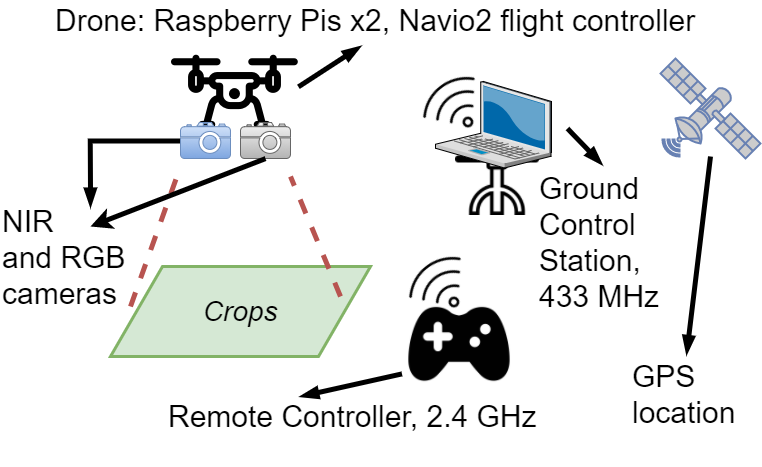
\includegraphics[scale=0.4]{images/drone_ndvi_scenario.png}
\caption{Illustration of the system as an overview}
\label{fig:scenario}
\end{figure}

A farmer would utilize the equipment for the purposes of capturing data. Specifically, the cameras on the drone will capture information about the farmer's crops, the remote controller is a failsafe to take over from autopilot, the GPS location georeferences each photo for the purpose of mapping, and the ground control station doubles as a mission planner and for the use of direct post-processing.\\

An example NDVI result is shown in Figure \ref{fig:vineyard_leaves}. Notice the different effects of the sun and shadows on the leaves.

\begin{figure}[H]
\begin{subfigure}{0.5\textwidth}
\centering
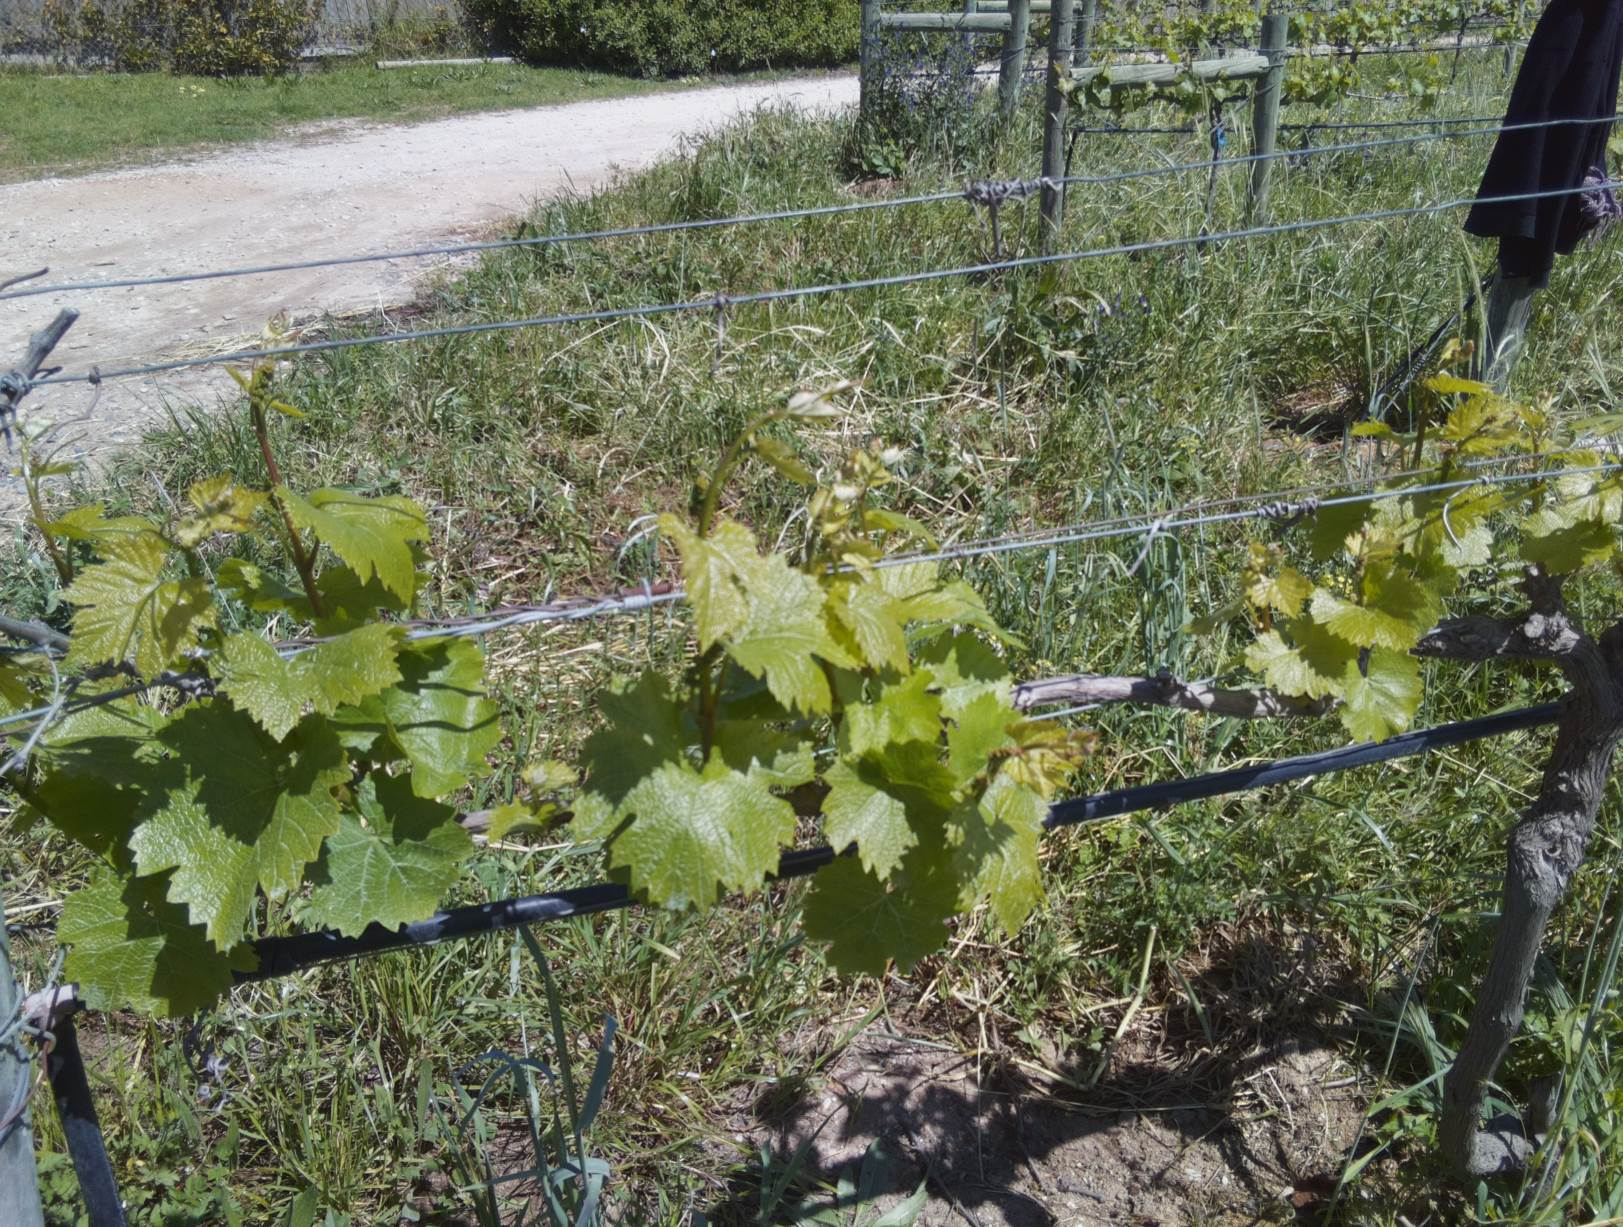
\includegraphics[scale=0.17]{images/rgb_leaves.jpg}
\caption{RGB image}
\end{subfigure}
\begin{subfigure}{0.5\textwidth}
\centering
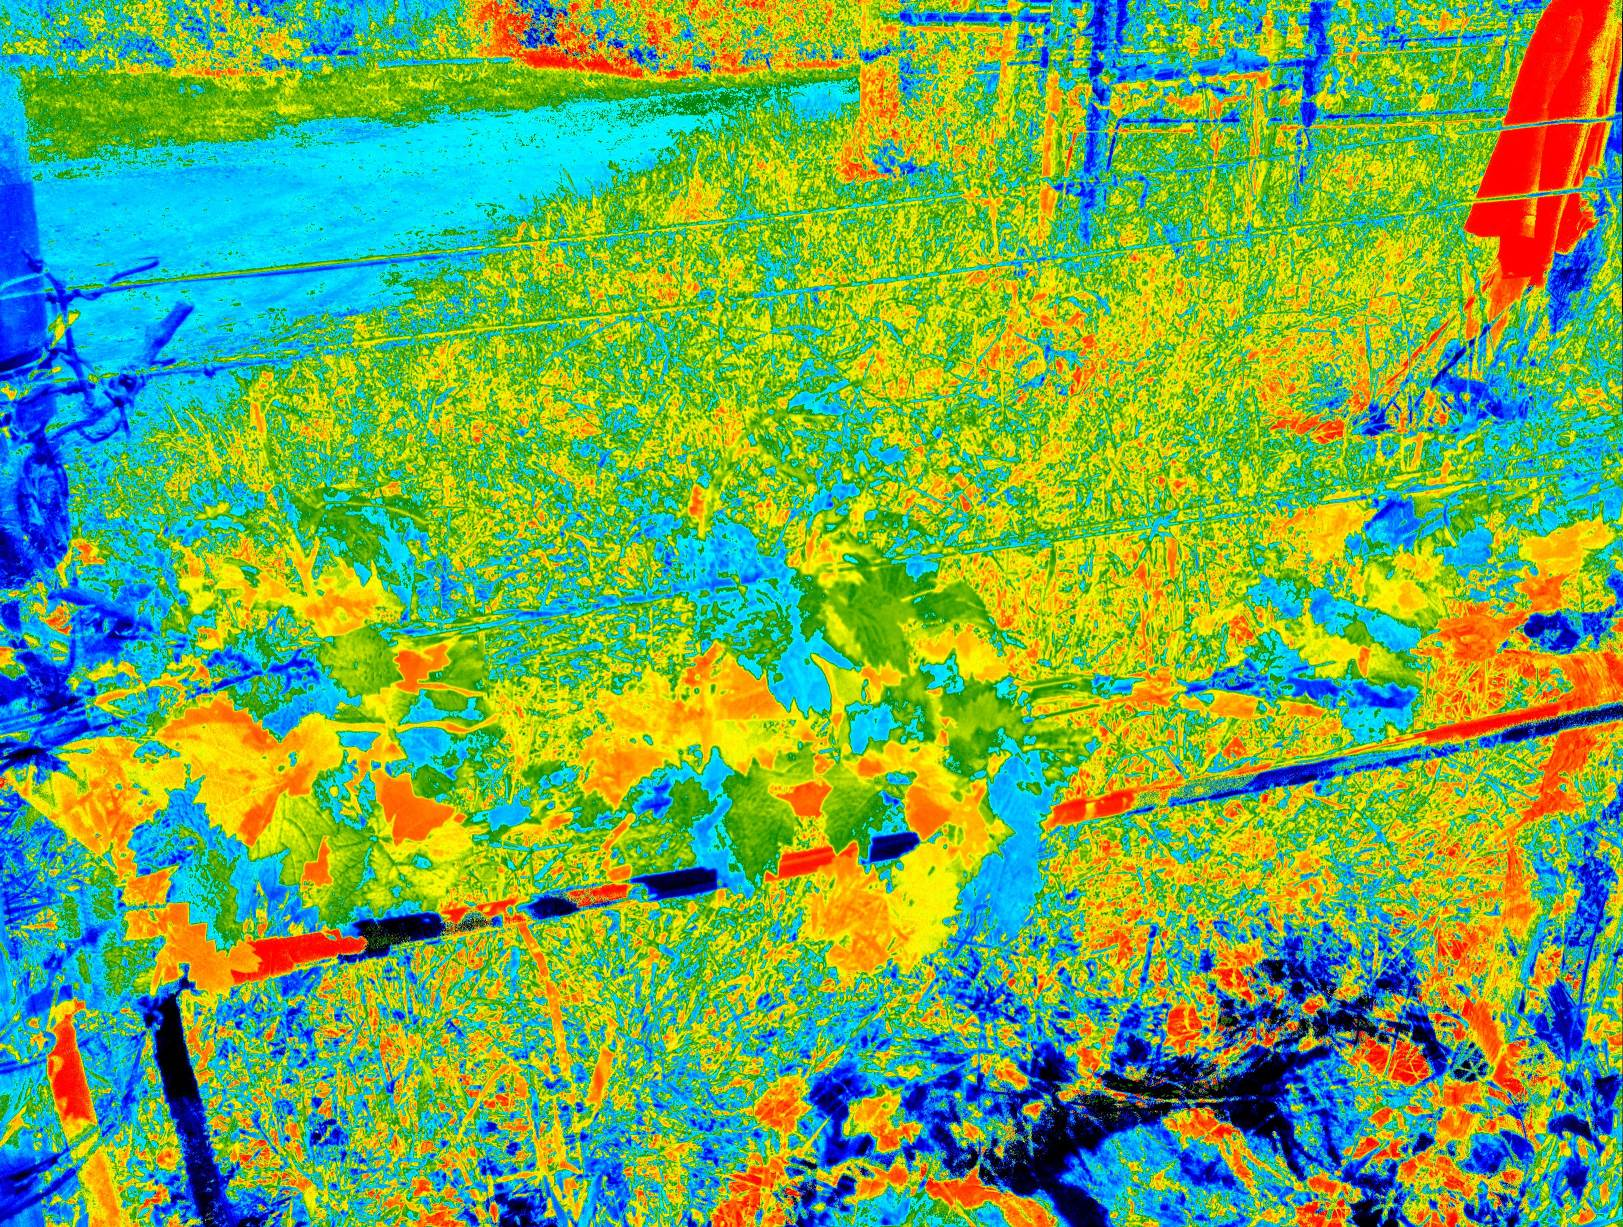
\includegraphics[scale=0.17]{images/ndvi_leaves.jpg}
\caption{Processed NDVI image}
\end{subfigure}
\caption{Closeup of vineyard leaves}
\label{fig:vineyard_leaves}
\end{figure}

%An implementation process of the system is illustrated in Figure \ref{fig:overview}. These processes will be expanded on and explained in the relevant chapters.
%
%\begin{figure}[H]
%\centering
%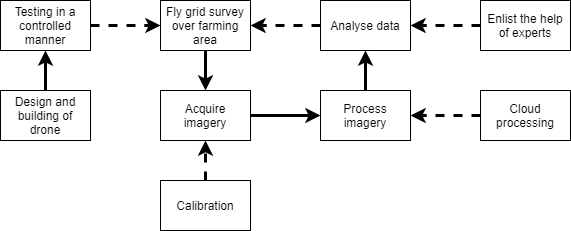
\includegraphics[scale=0.6]{images/thesis_overview.png}
%\caption{Implementation process}
%\label{fig:overview}
%\end{figure}
%
%Various drones, cameras, filters and processing techniques will be presented, as well as optimal choices depending on available resources.\\

A literature study will be investigated in Chapter 2, with drone design and construction in Chapter 3. Image acquisition and calibration will be handled in Chapter 4, and image processing in Chapter 5. Lastly, system integration and testing will be discussed in Chapter 6.